\documentclass[border=10pt]{standalone}

\usepackage[utf8]{inputenc}
\usepackage[english]{babel}
\usepackage{tikz}
\usetikzlibrary{positioning, arrows.meta, fit}

\tikzset{%
  neuron/.style={
    circle,
    draw,
    minimum size=1cm
  }
}

\definecolor{aogreen}{rgb}{0.0, 0.5, 0.0}
\definecolor{harvestgold}{rgb}{0.85, 0.57, 0.0}


\begin{document}
	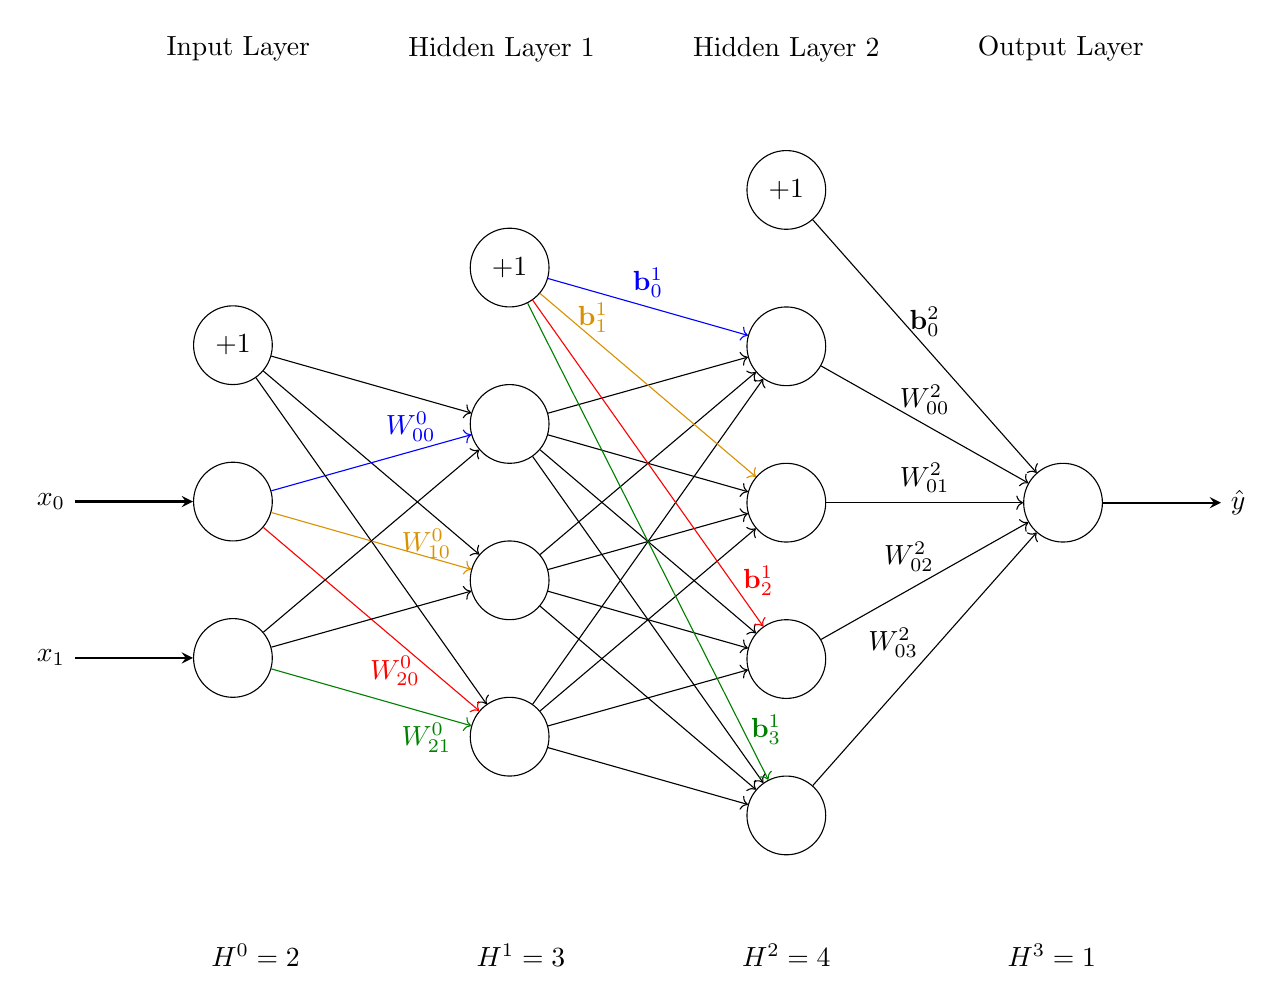
\begin{tikzpicture}
		% input layer
		\node[neuron] (a01) {};
		\node[neuron, yshift=4cm, below=of a01] (a00) {};
		\node[neuron, yshift=4cm, below=of a00] (b0) {$+1$};
		\node[xshift=-0.5cm, left=of a01] (x1) {$x_1$};
		\node[xshift=-0.5cm, left=of a00] (x0) {$x_0$};
		\draw[-stealth, thick] (x1) -- (a01);
		\draw[-stealth, thick] (x0) -- (a00);
		% hidden layer 1
		\node[neuron, yshift=-1cm, xshift=1.5cm, right=of a01] (a12) {};
		\node[neuron, yshift=4cm, below=of a12] (a11) {};
		\node[neuron, yshift=4cm, below=of a11] (a10) {};
		\node[neuron, yshift=4cm, below=of a10] (b1) {$+1$};
		% hidden layer 2
		\node[neuron, yshift=-1cm, xshift=1.5cm, right=of a12] (a23) {};
		\node[neuron, yshift=4cm, below=of a23] (a22) {};
		\node[neuron, yshift=4cm, below=of a22] (a21) {};
		\node[neuron, yshift=4cm, below=of a21] (a20) {};
		\node[neuron, yshift=4cm, below=of a20] (b2) {$+1$};		
		% output layer
		\node[neuron, xshift=1.5cm, right=of a21] (a30) {};
		\node[xshift=0.5cm, right=of a30] (y) {$\hat{y}$};
		\draw[-stealth, thick] (a30) -- (y);
		% description
		\node[above=of b2] (hl2) {Hidden Layer 2};
		\node[right=of hl2] (ol) {Output Layer};
		\node[left=of hl2] (hl1) {Hidden Layer 1};
		\node[left=of hl1] (il) {Input Layer};
		\node[below=of a23] (h2) {$H^2 = 4$};
		\node[right=of h2, xshift=1cm] (h3) {$H^3 = 1$};
		\node[left=of h2, xshift=-1cm] (h1) {$H^1 = 3$};
		\node[left=of h1, xshift=-1cm] (h0) {$H^0= 2$};
		% input layer connections
		\path [->] (b0) edge node [auto] {} (a10);
		\path [->] (b0) edge node [auto] {} (a11);
		\path [->] (b0) edge node [auto] {} (a12);
		% input0
		\path [->, draw=blue, text=blue] (a00) edge node [above, xshift=0.5cm, yshift=0.15cm] {$W^{0}_{00}$} (a10);
		\path [->, draw=harvestgold, text=harvestgold] (a00) edge node [above, xshift=0.7cm, yshift=-0.35cm] {$W^{0}_{10}$} (a11);
		\path [->, draw=red, text=red] (a00) edge node [below, yshift=-0.35cm, xshift=0.3cm] {$W^{0}_{20}$} (a12);
		% input1
		\path [->] (a01) edge node [auto] {} (a10);
		\path [->] (a01) edge node [auto] {} (a11);
		\path [->, draw=aogreen, text=aogreen] (a01) edge node [below, yshift=-0.2cm, xshift=0.7cm] {$W^{0}_{21}$} (a12);
		% hidden layer 1 connection
		\path [->] (a10) edge node [auto] {} (a20);
		\path [->] (a11) edge node [auto] {} (a20);
		\path [->] (a12) edge node [auto] {} (a20);
		\path [->, draw=blue, text=blue] (b1) edge node [above] {$\mathbf{b}^{1}_{0}$} (a20);
		\path [->] (a10) edge node [auto] {} (a21);
		\path [->] (a11) edge node [auto] {} (a21);
 		\path [->] (a12) edge node [auto] {} (a21);
 		\path [->, draw=harvestgold, text=harvestgold] (b1) edge node [above, yshift=0.55cm, xshift=-0.7cm] {$\mathbf{b}^{1}_{1}$} (a21);
		\path [->] (a10) edge node [auto] {} (a22);
		\path [->] (a11) edge node [auto] {} (a22);
		\path [->] (a12) edge node [auto] {} (a22);
		\path [->, draw=red, text=red] (b1) edge node [above, yshift=-1.8cm, xshift=1.4cm] {$\mathbf{b}^{1}_{2}$} (a22);				
		\path [->] (a10) edge node [auto] {} (a23);
		\path [->] (a11) edge node [auto] {} (a23);
		\path [->] (a12) edge node [auto] {} (a23);
		\path [->, draw=aogreen, text=aogreen] (b1) edge node [above, yshift=-2.7cm, xshift=1.5cm] {$\mathbf{b}^{1}_{3}$} (a23);
		% hiden layer 2 connection
		\path [->] (a20) edge node [above] {$W_{00}^{2}$} (a30);
		\path [->] (a21) edge node [above] {$W_{01}^{2}$} (a30);
		\path [->] (a22) edge node [above, xshift=-0.2cm] {$W_{02}^{2}$} (a30);
		\path [->] (a23) edge node [above, xshift=-0.4cm, yshift=-0.1cm] {$W_{03}^{2}$} (a30);
		\path [->] (b2) edge node [above] {$\mathbf{b}_{0}^{2}$} (a30);
	\end{tikzpicture}
\end{document}